\chapter{How to Show, Not Tell}

This lecture contains almost no mathematics in the ordinary sense, but it does have a formal spine. We are asked to think of prose as an inferential machine: do we hand the reader a conclusion, or do we hand the reader the evidence from which the conclusion may be drawn? The lecture proceeds in a carefully staged order. It begins with a deliberately bad passage, corrects the common slogan that telling is always bad, pauses for a short historical detour, and then develops six practical principles. We will keep that order, because the force of the lecture lies not only in what it says, but in how it brings us to each new step.

\begin{remark}
There is no literal blackboard mathematics here. Still, the lecture is structured tightly enough that a few schematic equations are useful. They are not claims about notation on a board; they are compact ways of writing the lecture's logic.
\end{remark}

\section{The Opening Failure}

We begin where the lecture begins: with a wilderness scene that is intentionally written the wrong way. A girl is said to be scared. The noises are said to be frightening. The ground is said to feel like a guardian. We are told the emotional outcome at every step, and yet the passage does not produce much feeling.

That is the right place to start, because the lecture is not first of all defining a slogan. It is diagnosing a failure. A sentence may name an emotion and still fail to make us experience it. A sentence may announce an atmosphere and still fail to create one.

\subsection{Question \& Answer}

The lecture pauses almost immediately to ask the question that should organize the whole chapter.

What is wrong with this picture?

The answer is that the prose supplies claims without evidence. Fear is asserted, but not dramatized. Atmosphere is asserted, but not earned. We are given verdicts where we need traces, pressures, sensations, or actions.

\begin{definition}
In the sense of this lecture, telling states a conclusion directly, whereas showing supplies the dramatic, sensory, or behavioral evidence from which the same conclusion may be inferred.
\end{definition}

The lecturer's sharpest compact formula, borrowed from K.\ M.\ Weiland, is worth writing out:

\begin{align}
\text{showing} &= \text{dramatizing},\\
\text{telling} &= \text{summarizing}.
\end{align}

This is already a useful correction. The trouble is not that summary exists; the trouble is that summary has been used where dramatic proof is needed.

\section{Showing, Telling, and the Reader's Inference}

Having staged the failure, the lecture immediately makes an important concession: telling is not inherently bad. If we turn ``show, don't tell'' into an absolute rule, we do not get better prose; we get bloated prose. Stories need compression, transition, and summary. They also need scenes in which the reader is allowed to live the moment from the inside.

The Secret Garden example is the lecture's first balancing move. We are told that Mary Lennox is disagreeable-looking and often ill, but the telling is immediately supported by visible proof: a thin face, a thin body, light hair, a sour expression. In other words, the lecture does not abolish telling. It insists that telling be anchored.

A useful way to write the lecture's basic logic is this:

\begin{equation}
\text{concrete detail} \leadsto \text{reader inference} \leadsto \text{emotion or judgment}.
\end{equation}

This same point is restated through Andrew Stanton's famous storytelling metaphor. We should not give the audience ``4'' if what we really want is active participation. We should give them ``2+2'' and let them perform the last step themselves. The exact phrasing in the transcript is slightly garbled, but the underlying idea is secure.

\begin{equation}
2+2 \to \text{audience inference}, \qquad 4 \to \text{premature closure}.
\end{equation}

That metaphor matters because it keeps showing from collapsing into ornament. The point is not to make prose more decorated. The point is to organize absence so that the reader works, but works willingly. The lecture insists that readers want to solve, deduce, and complete the picture. That is why implication is often more powerful than explanation.

\begin{figure}[h]
\centering
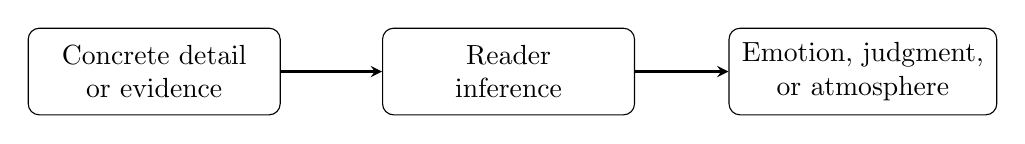
\begin{tikzpicture}[>=stealth]
\node[draw, rectangle, rounded corners, minimum width=3.2cm, minimum height=1.1cm, align=center] (a) at (0,0) {Concrete detail\\or evidence};
\node[draw, rectangle, rounded corners, minimum width=3.2cm, minimum height=1.1cm, align=center] (b) at (4.5,0) {Reader\\inference};
\node[draw, rectangle, rounded corners, minimum width=3.4cm, minimum height=1.1cm, align=center] (c) at (9.0,0) {Emotion, judgment,\\or atmosphere};
\draw[->, thick] (a) -- (b);
\draw[->, thick] (b) -- (c);
\end{tikzpicture}
\caption{A transcript-backed schematic of the lecture's central claim. We do not hand over the final verdict first; we hand over the evidence from which the verdict emerges.}
\end{figure}

\section{Why the Mantra Exists}

Before the lecture turns to technique, it pauses for a short historical explanation. That pause is important. Without it, the coming principles would feel like isolated workshop advice. With it, we understand the larger target.

The lecture locates the mantra in the rise of realism and in the attempt to make the novel feel less like authorial lecture and more like direct presentation. Percy Lubbock is cited as a key figure in popularizing the idea that fiction ought to be shown so that it seems to tell itself. Janice Hardy's practical restatement is equally useful: as long as it feels as though the character is thinking it, we are usually safe; when it sounds like the author stepping in to explain, we begin to lose the scene.

We can write the practical result as another schematic principle:

\begin{equation}
\text{author explanation} \downarrow \;\Longrightarrow\; \text{reader immersion} \uparrow.
\end{equation}

This is not a law. It is a tendency. The lecture itself will later insist that exposition and summary still have a place. But the historical detour clarifies the target: the real danger is not ``telling'' in some broad moral sense. The danger is authorial intrusion at moments when we most want the reader to inhabit the experience directly.

That is why the lecture now turns, in order, to six guiding principles.

\section{Evidence, Concrete Detail, and Sensory Specificity}

The first three principles belong together. They all answer the same question from different directions: if we cannot rely on naked assertion, what do we put on the page instead?

\subsection{Evidence Before Verdict}

The first move is the cleanest. When a narrator says someone is kind-hearted, or when a character decides a friend is guilty, or when a sentence declares that one character knows another likes him, we should ask the most basic question: what evidence produced that conclusion?

A thought-verb exercise cited in the lecture makes the same point by temporarily banning verbs such as ``knew,'' ``believed,'' ``wanted,'' and ``imagined.'' This is not because those verbs are forbidden in principle. It is because banning them for a moment forces us to uncover the scene that lies underneath the verdict.

\paragraph{Worked revision.} The lecture's example is ``Adam knew Gwen liked him.'' That sentence is efficient, but too efficient. The repair proceeds in a series of steps.

\begin{enumerate}
\item Start with the conclusion: ``Adam knew Gwen liked him.''
\item Ask what Adam actually perceives.
\item Replace the hidden judgment with repeated locker encounters, the heel mark on the painted metal, the smell of perfume, and the warm combination lock.
\item Stop once the reader can reach Adam's conclusion without being handed it in advance.
\end{enumerate}

Schematically, the revision looks like this:

\begin{align}
\text{``Adam knew Gwen liked him''}
&\xrightarrow{\text{revision}}
\text{locker} + \text{heel mark} + \text{perfume} + \text{warm lock}.
\end{align}

The lecture's principle is plain: instead of telling us that a character knows, give us the particulars that allow us to know.

\subsection{From the Abstract to the Concrete}

The second principle pushes the same method into emotional language. Instead of saying that Toby walked home happier than he had ever felt, the lecture prefers the goofy grin that will not leave his face, the buoyancy of his steps, the near-tripping energy of his body. Happiness is not denied. It is relocated from label to trace.

We can write the revision rule like this:

\begin{equation}
\text{abstract label} \xrightarrow{\text{revision}} \text{observable evidence}.
\end{equation}

The point is not to avoid abstraction because abstraction is somehow impure. The point is that abstract words often arrive too early. They tell us what to feel before the prose has created the conditions under which that feeling arises.

A few of the lecture's substitutions can be written schematically:

\begin{align}
\text{happy} &\xrightarrow{\text{showing}} \text{goofy grin} + \text{buoyant movement},\\
\text{eerie} &\xrightarrow{\text{showing}} \text{the forest hums with the cries of children long dead}.
\end{align}

The ``eerie forest'' example is especially useful. ``The dark forest felt eerie'' is not false. It is merely underpowered. The revision does not argue with the adjective. It earns it.

\subsection{Can the Camera See It?}

The lecture's most operational test is a question: can the camera see it? That question is not complete by itself, because writing also has smell, touch, taste, and sound at its disposal. Still, it is a strong first filter. If the camera cannot see it, we should ask whether the prose has supplied any concrete sensory evidence at all.

This produces a third schematic rule:

\begin{equation}
\text{cause statement} \xrightarrow{\text{showing}} \text{visible or sensory effect}.
\end{equation}

The Jerry Jenkins examples make the point neatly:

\begin{align}
\text{cold}
&\xrightarrow{\text{showing}}
\text{collar up} + \text{scarf tightened} + \text{hands in pockets} + \text{face turned from wind},\\
\text{blindness}
&\xrightarrow{\text{showing}}
\text{white cane feeling for the bench},\\
\text{late fall}
&\xrightarrow{\text{showing}}
\text{leaves crunch beneath the feet}.
\end{align}

The lecture then widens the principle. Specificity is not only a matter of visibility. Delilah Dawson's market scene becomes stronger when it moves beyond rugs and spices and gives us cinnamon, coffee, silken tassels, and powdered saffron. The prose becomes more immersive because the detail becomes more local and more sensory.

At this point the lecture adds a subtle but important correction. If we merely substitute one stock image for another, we are still in trouble. A funeral in the rain may be technically visual, but it may also be inert because it is so expected. Hence the Gail Carson Levine examples: change the setting, introduce a gravestone inscription that does not make immediate sense, let the scene resist cliché. We do not want detail in the abstract. We want the right detail, in the right place, under the pressure of the scene.

\section{Beyond Body Language}

The fourth principle is corrective. Once writers are told to ``show,'' they often grab the quickest available shorthand: clenched fists, crossed arms, gritted teeth, tapping fingers, racing hearts, rolling stomachs. The lecture does not deny that such gestures can communicate mood. It insists only that they are often too blunt.

\subsection{Question \& Answer}

Is body language enough?

Usually not. It may tell us that something is happening, but it often fails to tell us what precisely is happening. Anger may look like frustration, slight, jealousy, panic, or grief in outward gesture. The lecture's point is that stock physical signals often flatten emotional nuance rather than deepen it.

Robin Patchen's before-and-after example is the lecture's best extended demonstration. In the first version, Mary looks at the clock, her heart leaps, her stomach rolls, and we are told something is wrong. At first glance this appears to be showing. But the lecture argues that it is still melodramatic because it remains too dependent on generic internal alarms.

The revised version is better not because it avoids the body entirely, but because it moves into sequence, setting, and thought. Sunlight comes through the open window. Mary sits up. She sees the clock. She realizes the baby has slept through the night. Then memory intrudes: Billy. Then action follows: she flips the covers back, snatches the robe, repeats the doctor's reassurance to herself. The scene stops naming panic and instead behaves panicked.

The lecture condenses this into a small causal chain:

\begin{equation}
\text{thoughts} \to \text{emotions} \to \text{actions}.
\end{equation}

This is one of the most useful formal statements in the whole lecture. It tells us where to look when a scene feels emotionally thin. If we jump straight to bodily shorthand, we may miss the thought-process that actually generates the action. If we restore the thought-process, the emotion begins to emerge with much finer resolution.

We can summarize the revision like this:

\begin{enumerate}
\item Replace generic visceral signals with the local sequence of perception and memory.
\item Let setting participate: the sunlight, the clock, the room, the robe.
\item Let verb choice carry force: ``flipped'' and ``snatched'' are stronger than neutral motion verbs.
\item Use syntax itself as a form of showing; short units and interrupted thought can perform urgency.
\end{enumerate}

That is why the lecture advises us to slow down emotional scenes. If the scene matters, we should not race past the character's thought. We should let the thought produce the feeling and the feeling produce the action.

\section{Dialogue, Telegraphing, and Subtext}

The fifth principle extends the same logic into speech. Dialogue can prove a character's feeling or personality directly, without explanatory help, provided we trust it to do the work.

The lecture's humorous example makes the point quickly. Instead of writing that Mary was angry at Bob, we can let Mary shout at him. Once the words themselves carry anger, an additional adverb such as ``angrily'' often becomes redundant.

That redundancy is the lecture's next target. A tag or adverb is not always wrong. It is wrong when it merely restates what the dialogue has already made obvious.

\subsection{Question \& Answer}

When does dialogue start telegraphing instead of showing?

Dialogue begins telegraphing when narration announces a motive or intention that the spoken exchange already conveys. If we write that he tried to be diplomatic, and then the line itself is patient and conciliatory, we have doubled the information. If we write that she is changing the subject, and then she immediately moves the conversation elsewhere, we have explained what the reader could already infer.

We may write the contrast schematically:

\begin{align}
\text{dialogue} + \text{redundant explanation} &\to \text{telegraphing},\\
\text{dialogue} + \text{precise action beat} &\to \text{sharper subtext}.
\end{align}

The lecture's revised exchange shows the difference. Instead of explanatory labels, we get a small action beat and a selective tag: he pinches the bridge of his nose; she whispers. The words themselves continue to carry most of the burden, but the surrounding details sharpen the social pressure of the moment.

The advice then widens once more. If we want to learn how to carry emotion through dialogue, it can help to draft the scene as though it were a play or screenplay. That forces us to rely less on authorial explanation and more on the force, rhythm, and implication of what is said. The lecture invokes Oscar Wilde here for precisely that reason. In the cited exchange between Algernon and Jack, the emotional temperature is audible in the words. We do not need the narrator to stop and decode the feeling for us.

The practical rule is simple: let the spoken line, the selected beat, and the social context do the work before we reach for explanation.

\section{Narrative Voice, Pacing, and the Return to the Opening}

The sixth principle makes the chapter larger than sentence-by-sentence repair. Showing is not only a matter of swapping out one adjective or tag. It is also a matter of point of view and pacing.

The lecture first handles narrative voice. When we say that a man was rude and inconsiderate, or that a woman was uncomfortable, or that a house was huge, or that a character was hungry, we are again starting from verdict. The better alternative is not merely to attach random detail. It is to filter the detail through a perspective and let the line arrive with voice.

This is why the lecture likes examples such as the stroller on the bus, the woman stiffening in an embrace, the kitchen large enough to house the whole family, or the soup nearly inhaled. These are not only more vivid. They carry attitude. They come from a mind positioned inside the scene.

The same logic applies to exposition. Janice Hardy's distinction between information given for the reader's benefit and information given for the character's benefit is crucial. A sentence that exists only to brief the audience often sounds external to the scene. A sentence that arises from what the character would naturally notice, fear, or say remains inside the fiction.

The lecture's restaurant comparison makes this vivid. The same basic setup changes entirely depending on whether the point of view belongs to a bland observer, a Navy SEAL, or a frightened girl. The facts are not wholly different. The world is being filtered differently. Rain is no longer just weather; it becomes rounds from an Uzi, or a blur that hides the world outside. The envelope is no longer a neutral object; it becomes pressure.

At this stage the lecture restores telling to its proper place. The final claim is not ``show always.'' It is ``show, don't just tell.'' Telling remains one of the writer's pacing tools. We may write the lecture's closing balance like this:

\begin{equation}
\text{telling} + \text{specific detail} = \text{an acceptable blend when pacing requires it}.
\end{equation}

And we can compress the pacing rule into a practical table.

\begin{table}[h]
\centering
\begin{tabular}{|p{0.42\textwidth}|p{0.42\textwidth}|}
\hline
\textbf{Tell or blend when we need speed} & \textbf{Show when we need presence} \\
\hline
Bridges from point A to point B & Emotions \\
\hline
Routines, time passing, repeated conversations & Sensations: sight, sound, smell, taste, touch \\
\hline
Broad exposition or occasional backstory & Assumptions and judgments about people or places \\
\hline
Some world-building summaries & Dialogue tone, motive, and conversational intention \\
\hline
Character thought in broad sweep & The concrete traces from which feeling is inferred \\
\hline
\end{tabular}
\caption{The lecture's closing pacing rule. Telling is not abolished; it is allocated.}
\end{table}

This is where the discussion of strong narrative voice enters. Alexi Harrow's praise of exposition-rich fiction matters because it prevents us from turning ``show, don't tell'' into a rule against all narrated intelligence. Strong prose can tell magnificently if voice carries tension, attitude, and pressure. The cited opening of The Space Between Worlds is not offered as a rejection of showing, but as proof that narrated exposition can still be charged when it is saturated with a living point of view.

Finally, the lecture returns to the wilderness scene with which it began. This return is structurally essential. We do not merely leave with a list of rules; we see the original problem solved. The repaired passage from Delia Owens does not simply announce fear leaving the girl. It lets the land catch her when she stumbles. It lets the pain seep away like water into sand. It lets the marsh become mother. That is the crucial difference. The transformation is no longer reported from outside. It is enacted through image, action, and voice.

\section{Summary}

We can now state the lecture's central lesson in its strongest form. Showing is not the banishment of telling. It is the discipline of making the reader do the last necessary step.

When a sentence feels weak, the lecture gives us a sequence of questions to ask.

\begin{itemize}
\item Have we supplied a verdict before we have supplied evidence?
\item Have we named an emotion where a concrete trace would do better?
\item Can the camera see what we have written, or at least can the senses register it?
\item Are we leaning on stock body language instead of thought, setting, and action?
\item Are we explaining dialogue that already explains itself?
\item Is exposition serving the character's point of view, or merely briefing the reader?
\end{itemize}

The lecture's mature conclusion is therefore neither austere nor slogan-driven. We show when we want presence, inference, and emotional participation. We tell when we need pace, compression, or broad sweep. The craft lies in knowing which mode the moment requires, and in refusing to hand the reader ``4'' when the scene will be stronger if we give them ``2+2.''